\documentclass[aspectratio=169]{beamer}
\usetheme{Madrid}
\usecolortheme{dolphin}

\usepackage{booktabs}
\usepackage{xcolor}
\usepackage{listings}
\usepackage{graphicx}
\usepackage{tikz}
\usetikzlibrary{positioning,arrows.meta}
\usepackage{amsmath}

\definecolor{myblue}{RGB}{41,98,158}
\definecolor{mygreen}{RGB}{46,125,50}
\definecolor{myred}{RGB}{183,28,28}
\definecolor{myorange}{RGB}{230,126,34}
\definecolor{codebg}{RGB}{13,17,23}
\definecolor{codefg}{RGB}{201,209,217}
\definecolor{mygray}{RGB}{100,100,100}

\setbeamercolor{frametitle}{bg=myblue,fg=white}
\setbeamercolor{structure}{fg=myblue}
\setbeamertemplate{navigation symbols}{}
\setbeamertemplate{footline}{}

\lstset{
  backgroundcolor=\color{codebg},
  basicstyle=\ttfamily\scriptsize\color{codefg},
  keywordstyle=\color{cyan},
  commentstyle=\color{gray!80},
  language=C, frame=none, tabsize=2,
  breaklines=true, showstringspaces=false
}

\title[PhD Year 3 Plan]{PhD Year 3 Plan --- Pre-EOY Alignment}
\subtitle{Specification Synthesis, Infrastructure, and Quality for LLM-Assisted BMC}
\author[Weiqi Wang]{Weiqi Wang}
\institute[]{Supervisors: Prof.\ Lucas Cordeiro \& Dr.\ Marie Farrell}
\date{\today}

\begin{document}

% ── 1. Title ──────────────────────────────────────────────────────────────────
\begin{frame}
  \titlepage
\end{frame}

% ── 2. Where I Am — Year 2 Recap ──────────────────────────────────────────────
\begin{frame}{Where I Am --- Year 2 Recap}

\textbf{Three first-author lines:}
\medskip

{\small\renewcommand{\arraystretch}{1.35}
\begin{tabular}{p{0.20\textwidth}p{0.48\textwidth}p{0.22\textwidth}}
\toprule
\textbf{Project} & \textbf{Direction} & \textbf{Status} \\
\midrule
\textcolor{mygreen}{\checkmark}\ \textbf{SpecVerify} &
LLM-driven NL $\rightarrow$ ESBMC spec synthesis &
\textcolor{mygreen}{RE'25 published} \\
\textcolor{myorange}{$\circlearrowright$}\ \textbf{Frame\_func} &
ESBMC function contract framework $+$ Lean soundness &
\textcolor{myorange}{ASE'26 under review} \\
\textcolor{myblue}{$\bullet$}\ \textbf{LLM4Harness} &
Diagnosing what LLMs miss when writing CBMC harnesses &
\textcolor{myblue}{In preparation} \\
\bottomrule
\end{tabular}}

\bigskip
\textbf{Two collaborations:}
\begin{itemize}\small
  \item \textcolor{myorange}{$\circlearrowright$}\ \textbf{ConVer} (co-first w/ Pirzada, Charalambous) ---
        function contract framework integration into compositional pipeline.
        \textcolor{myorange}{ASE'26 under review.}
  \item \textbf{VerIbmc} (third author) --- LLM synthesises loop invariants;
        validated via my loop-invariant check infrastructure. In submission.
\end{itemize}

\bigskip
{\small\color{mygray}
Backup plan if ASE'26 rejection: Frame\_func can pivot to tool paper; ConVer stays research track.}

\end{frame}

% ── 3. Thesis Pipeline ────────────────────────────────────────────────────────
\begin{frame}[shrink=5]{Thesis Pipeline --- Where Each Artifact Sits}
\begin{center}
  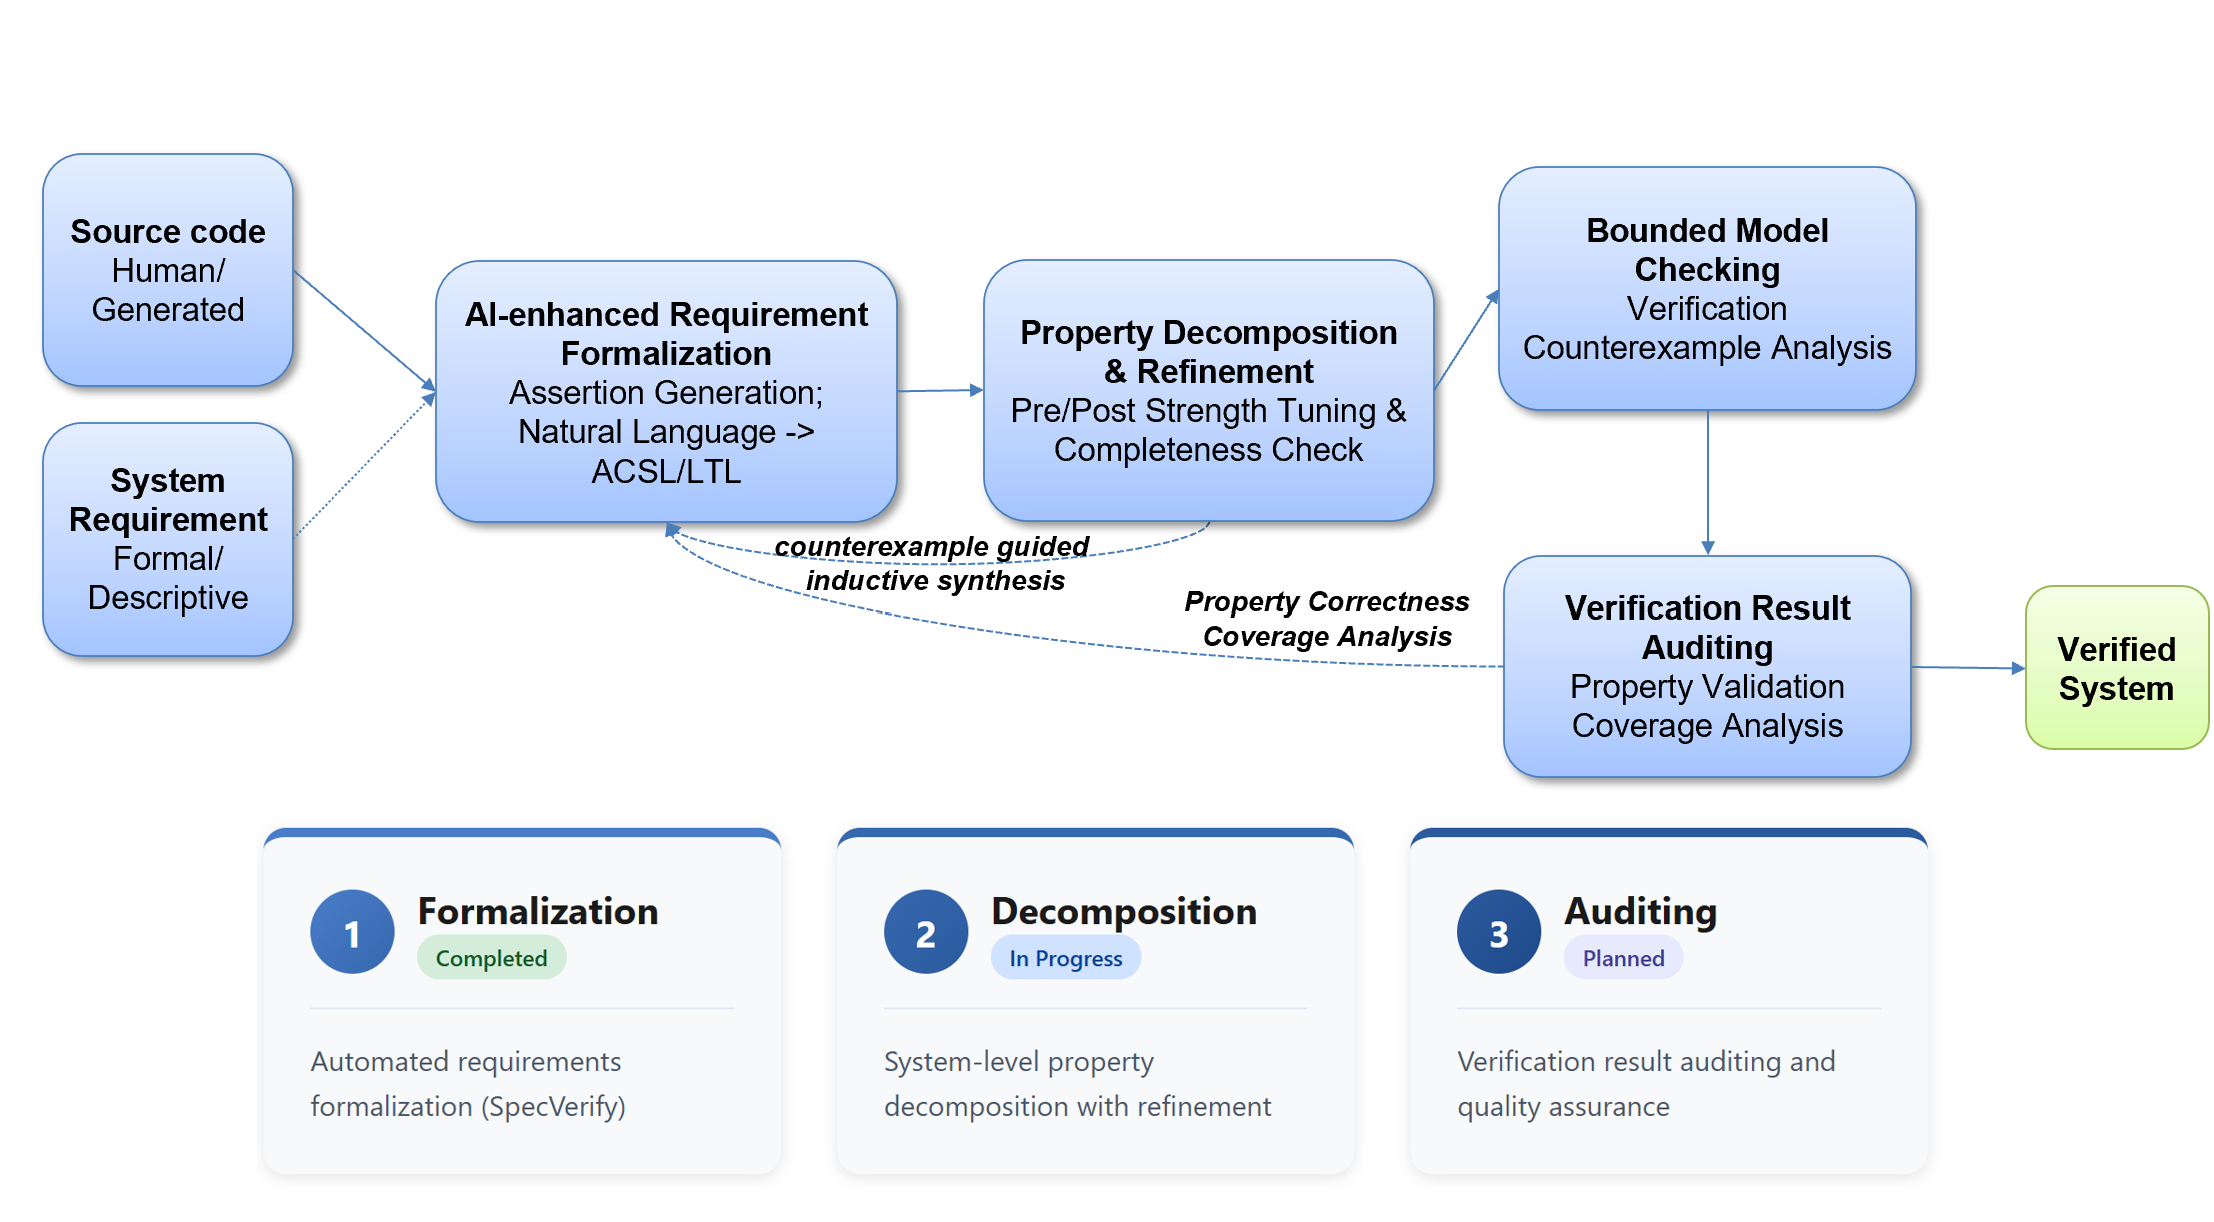
\includegraphics[width=0.85\textwidth]{figures/thesis_pipeline.png}
\end{center}
{\small\color{myblue}
\textbf{Throughline:} \emph{Better specifications $\rightarrow$ better infrastructure $\rightarrow$
trustworthy LLM-assisted BMC.} Year 3 builds a multi-oracle quality gate on top of
Year 2's contract framework $+$ diagnostic taxonomy.}
\end{frame}

% ── 4. Year 1: SpecVerify ─────────────────────────────────────────────────────
\begin{frame}{Year 1 --- SpecVerify}

\textbf{Direction:} Can LLMs translate NL requirements into ESBMC assertions?

\bigskip
\begin{itemize}
  \item NL $\rightarrow$ ESBMC pipeline on CPS benchmarks
  \item Hit a \textcolor{myred}{flat-assertion ceiling} on temporal / quantified properties
  \item \textbf{This ceiling is what motivated Year 2's move to function contracts}
\end{itemize}

\bigskip
\textbf{Status:} \textcolor{mygreen}{Published at RE'25} (first author)

\end{frame}

% ── 5. Frame_func ─────────────────────────────────────────────────────────────
\begin{frame}{Year 2 Main 1 --- Frame\_func}

\textbf{Direction:} Lift ESBMC from \emph{flat assertions} $\rightarrow$ \emph{function contracts} ---
the modular verification missing piece.

\bigskip
\begin{itemize}
  \item Complete \texttt{requires} / \texttt{ensures} / \texttt{assigns} pipeline in ESBMC
  \item \textcolor{mygreen}{\textbf{Lean 4 soundness}} --- machine-checked end-to-end
  \item Validated on industrial cases (ANSSI X.509, FreeRTOS \texttt{heap\_1})
\end{itemize}

\bigskip
\textbf{Status:} \textcolor{myorange}{ASE'26 under review}
\quad·\quad Backup: tool paper track
\quad·\quad \emph{Year 2 technical core}

\end{frame}

% ── 6. LLM4Harness (condensed) ────────────────────────────────────────────────
\begin{frame}{Year 2 Main 2 --- LLM4Harness \textcolor{mygray}{\small(Year 3 pilot)}}

\textbf{Two pivots got us here:}

\medskip
\begin{center}
  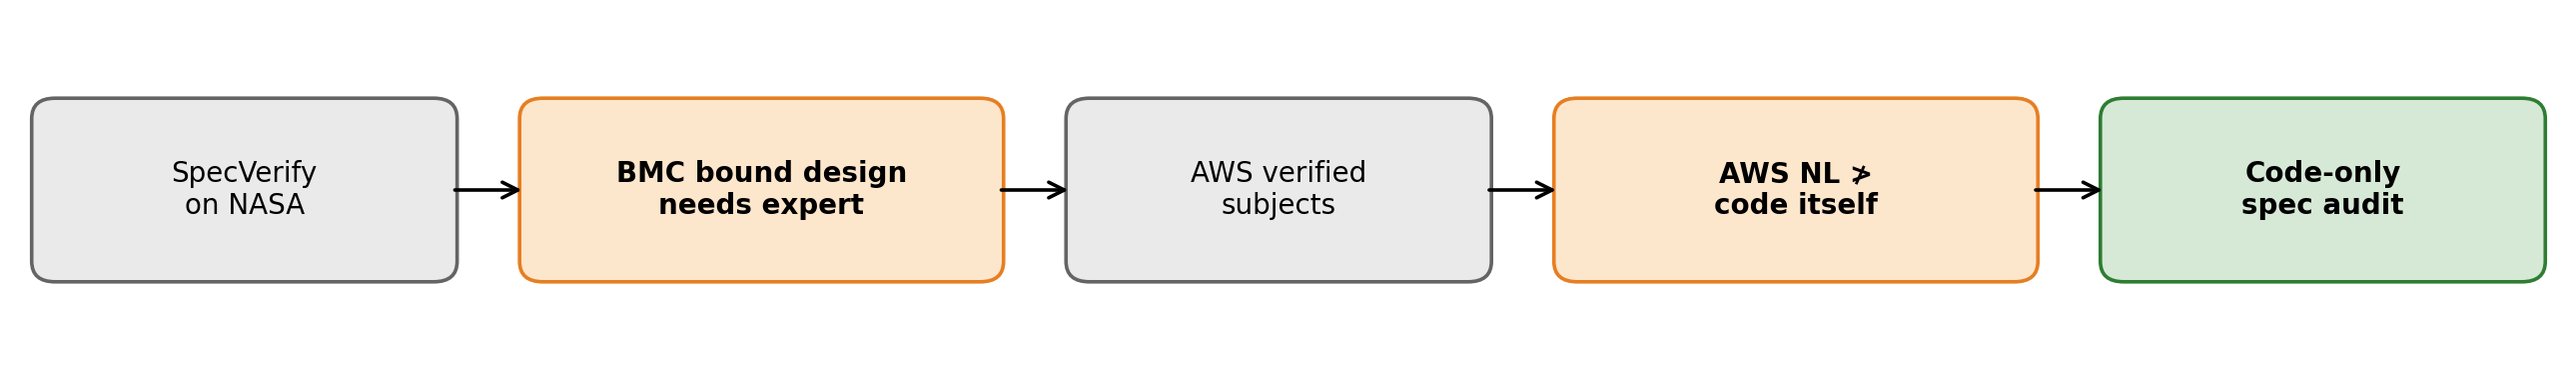
\includegraphics[width=0.95\textwidth]{figures/llm4harness_pivot.png}
\end{center}

\medskip
\textbf{Three findings that bridge to Year 3:}
\begin{itemize}\small
  \item Pass rate \textbf{94\%}, recall vs.\ expert GT only \textbf{47\%}
  \item \textcolor{myred}{\textbf{56\% of misses are structural}} ---
        tool-idiomatic, not function misunderstanding
  \item Text prompting \emph{does not help}; one same-family example $+$\textbf{9pp}
\end{itemize}

\smallskip
{\footnotesize\color{mygray}
recall $=$ \#matched assertions $/$ \#GT assertions \;·\;
structural $=$ tool-idiom categories (validity predicates, frame conditions, length invariants)}

\smallskip
\textbf{Status:} pilot experiments running; draft $\sim$30\%, first author
\quad·\quad Conference scope (FSE / ASE / ICSE) --- venue open

\end{frame}

% ── 7. ConVer ─────────────────────────────────────────────────────────────────
\begin{frame}{Year 2 Collaboration --- ConVer \textcolor{mygray}{\small(co-first)}}

\textbf{Direction:} Top-down compositional verification with LLM-synthesised contracts ---
making large C programs tractable for BMC.

\bigskip
\textbf{My role:} contract framework integration $+$ ESBMC backend ---
this is where Frame\_func's \texttt{frame\_enforcer} pays off in a second project.

\bigskip
\textbf{Co-first authors:} Pirzada, \textbf{Wang}, Charalambous

\bigskip
\textbf{Status:} \textcolor{myorange}{ASE'26 under review} (research track)
\quad·\quad Thesis: appendix

\end{frame}

% ── 8. Year 3 Main Project ────────────────────────────────────────────────────
\begin{frame}[shrink=5]{Year 3 Main Project --- BMC Spec Audit}

\textbf{Goal:} scalable spec quality gate for LLM-generated ESBMC function contracts ---
the \emph{paired solution} to LLM4Harness's diagnosis.

\smallskip
\begin{center}
  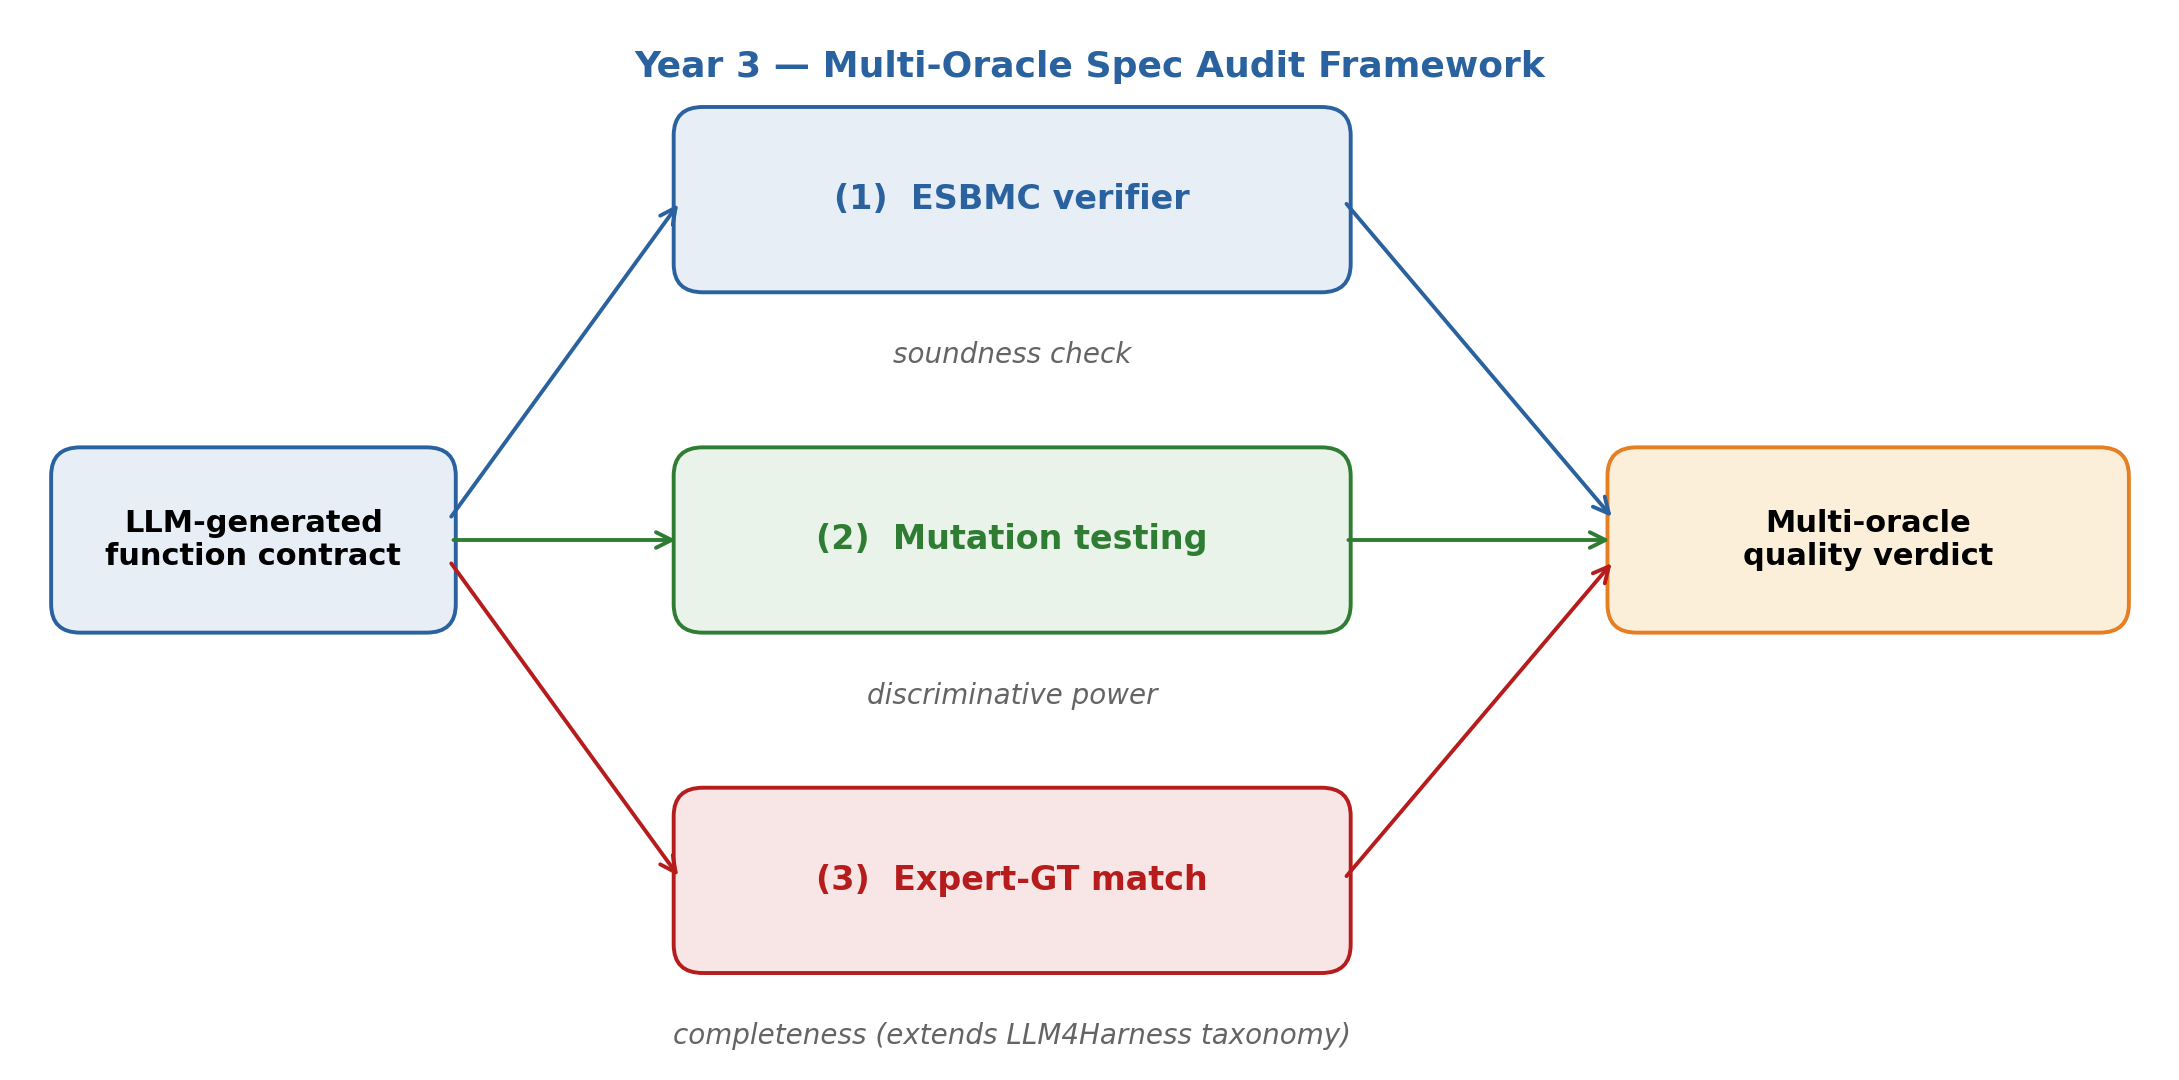
\includegraphics[width=0.74\textwidth]{figures/multi_oracle.png}
\end{center}

\smallskip
{\footnotesize\color{mygray}
Mutation testing $=$ checks if the contract rejects buggy mutants of the function
(i.e., is the spec strong enough to catch real bugs?)}

\smallskip
{\small\textbf{Setup:}
3 LLMs $\times$ $\sim$150 industrial functions
(s2n-tls, aws-c-common, ConVer, Frame\_func) \;·\; code-only framing
\;·\; reuses Year 2 infrastructure}

\end{frame}

% ── 9. Year 3 Timeline + Risks ────────────────────────────────────────────────
\begin{frame}[shrink=5]{Year 3 Timeline --- Three Pacing Options}

\begin{center}
  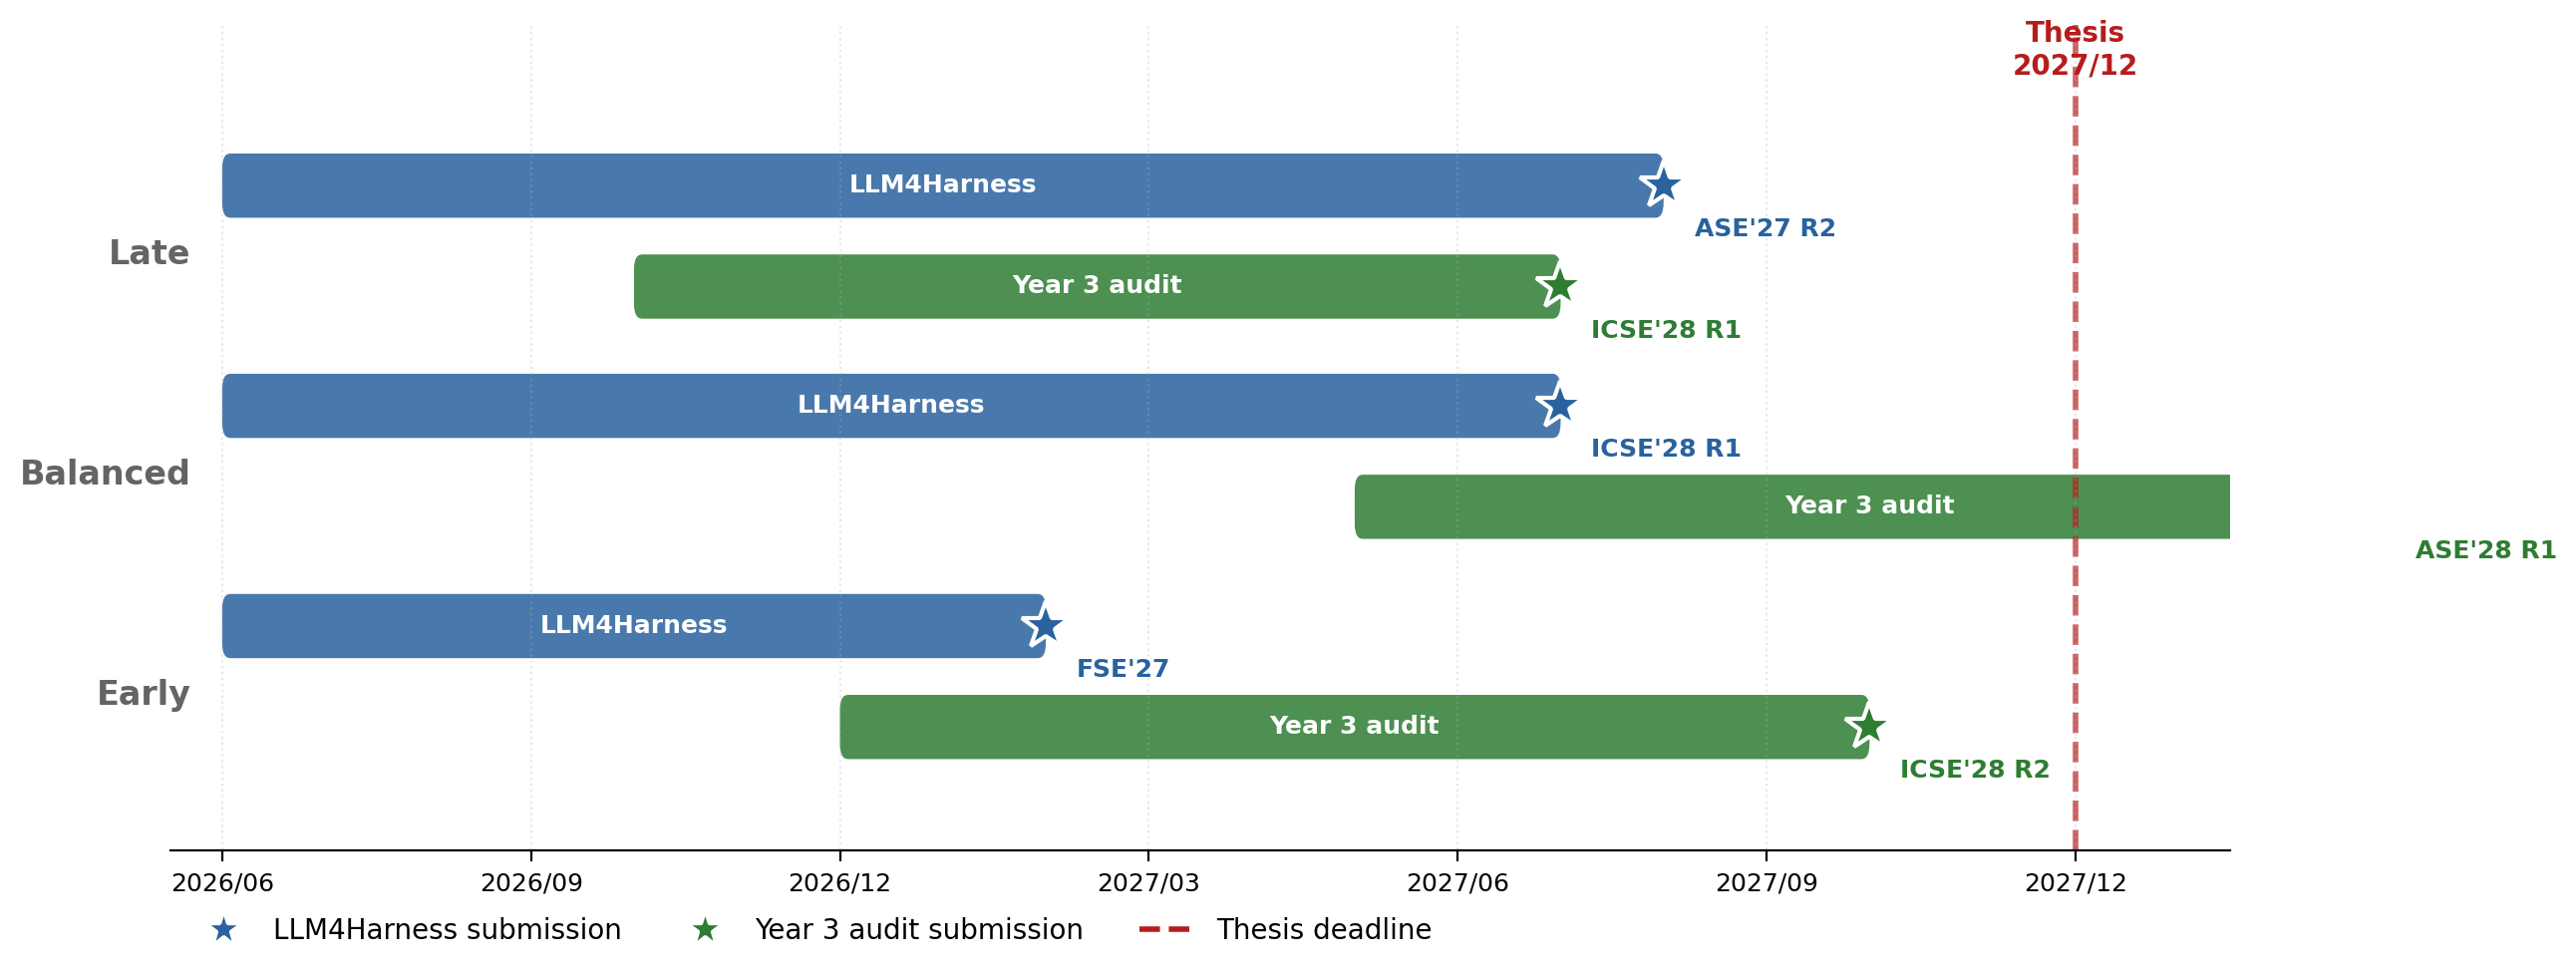
\includegraphics[width=0.86\textwidth]{figures/year3_timeline.png}
\end{center}

\smallskip
\begin{columns}[T]

\column{0.50\textwidth}
{\small\textbf{Reading the chart:}\\
\textbullet\ \textcolor{myblue}{\textbf{Early}} --- fastest LLM4Harness, longest audit runway\\
\textbullet\ \textcolor{myblue}{\textbf{Balanced}} --- audit submission \textbf{slips past thesis}\\
\textbullet\ \textcolor{myblue}{\textbf{Late}} --- audit done before thesis writing}

\column{0.47\textwidth}
\begin{block}{\textcolor{mygray}{\small Risks (acknowledged)}}
{\footnotesize
\textbullet\ Mutation oracle saturation (equivalent mutants)\\
\textbullet\ Inter-rater $\kappa$ on extended taxonomy\\
\textbullet\ Frame\_func rejection $\rightarrow$ tool paper rework ($\sim$3 mo delta)}
\end{block}

\end{columns}

\vspace{2em}

\end{frame}

% ── 10. Decision 1 — Year 3 Framing ───────────────────────────────────────────
\begin{frame}{Decision 1 --- Year 3 Framing \quad\textcolor{myred}{\small[need input]}}

Two candidate framings for the Year 3 main project:

\bigskip
\begin{columns}[T]

\column{0.48\textwidth}
\begin{block}{\textbf{Option A: Code-only Spec Audit}}
{\small
\emph{``From code alone, can LLMs reconstruct
expert-quality contracts?''}}

\medskip
{\small
\textcolor{mygreen}{\textbf{Pro:}} clean continuation of LLM4Harness;
benchmark fully aligned\\[4pt]
\textcolor{myred}{\textbf{Con:}} narrower thesis claim (NL-sparse only);
must explain why Year 3 abandons NL after Year 1 used it}
\end{block}

\column{0.48\textwidth}
\begin{block}{\textbf{Option B: Spectrum Framing}}
{\small
\emph{``BMC adaptation across the NL availability spectrum.''}}

\medskip
{\small
\textcolor{mygreen}{\textbf{Pro:}} broader thesis claim --- unifies SpecVerify,
LLM4Harness, and Year 3 audit under one arc\\[4pt]
\textcolor{myred}{\textbf{Con:}} writing risk --- requires intro rewrite;
spectrum claim must hold across all three chapters}
\end{block}

\end{columns}

\bigskip
\textbf{Open questions:}
\begin{itemize}\small
  \item Which framing fits your view of the thesis?
  \item Can we test Option B with a 200-word intro draft before committing?
\end{itemize}

\end{frame}

% ── 11. Decision 2 — LLM4Harness Pacing ───────────────────────────────────────
\begin{frame}{Decision 2 --- LLM4Harness Submission Pacing
\quad\textcolor{myred}{\small[need input]}}

\textbf{Setup:} venue not pre-committed; conference (FSE / ASE / ICSE) more likely than journal.

\smallskip
{\small\color{mygray}
Slide 9's three execution paces map to different venue windows.
Each row below is the same option, viewed from the submission side.}

\medskip
{\small\renewcommand{\arraystretch}{1.5}
\begin{tabular}{p{0.16\textwidth}p{0.74\textwidth}}
\toprule
\textbf{Pacing} & \textbf{Trade-off} \\
\midrule
\textbf{Early} &
Reviewer feedback \emph{before} audit work; rushed revision risk if R1 returns major comments \\
\textbf{Balanced} &
Spreads thesis load; \textbf{audit submission slips past thesis deadline} (ASE'28 R1) \\
\textbf{Late} &
More polish on LLM4Harness; revision concurrent with thesis writing in 2027/09--12 \\
\bottomrule
\end{tabular}}

\bigskip
\textbf{Open questions:}
\begin{itemize}\small
  \item Which pacing minimises thesis-end pressure (2027/09--12)?
  \item Should I commit now or wait for ASE'26 outcome (Frame\_func)?
\end{itemize}

\end{frame}

% ── 12. Decision 3 — RQ Allocation ────────────────────────────────────────────
\begin{frame}{Decision 3 --- LLM4Harness vs.\ Year 3 RQ Allocation
\quad\textcolor{mygray}{\small[can defer]}}

\textbf{LLM4Harness paper currently has four RQs:}
\begin{itemize}\small
  \item RQ1: Diagnosis (47\% recall, 56\% structural \textcolor{mygray}{--- see Slide 6})
  \item RQ2: Prompting vs.\ examples ($+$9pp)
  \item RQ3: Transfer mechanism decomposition (\emph{generic} vs.\ \emph{predicate vocab})
  \item RQ4: Cross-library replication
\end{itemize}

\bigskip
\textbf{Question:} should RQ3 (transfer mechanism) belong to:
\begin{itemize}\small
  \item[(a)] LLM4Harness paper (current placement)
  \item[(b)] Year 3 audit work --- would refocus LLM4Harness on \emph{diagnosis only}
\end{itemize}

\bigskip
{\small\color{mygray}
Decision can wait until Year 3 pilot results (2026/12 or later).
Flagging now to align supervisors on long-term thesis structure.}

\end{frame}

% ── 13. Closing ───────────────────────────────────────────────────────────────
\begin{frame}{Closing \& Open Questions}

\textbf{Year 2 status:} 3 first-author lines $+$ 2 collaborations\\
\textbf{Year 3 plan:} multi-oracle BMC spec audit\\
\textbf{Thesis target:} 2027/12 submission

\bigskip
\textbf{Immediate questions for this meeting:}
\begin{enumerate}\small
  \item \textbf{Year 3 framing:} Option A or Option B?
        \emph{(need decision before EOY)}
  \item \textbf{LLM4Harness pacing:} early / balanced / late?
        \emph{(can wait for ASE'26 outcome)}
  \item \textbf{Year 2 retrospective for EOY:} anything missing or
        underweighted in this deck?
\end{enumerate}

\bigskip
\begin{center}
{\large Thank you.}
\end{center}

\end{frame}

\end{document}
